\chapter{Preliminaries}
\section{Class-D Amplifier}
A Class-D Amplifier, also known as "digital-amplifier" is a very efficient design of a power amplifier most commonly used in audio applications. The main principal is based on a switching output stage (often constructed with \acrshort{mosfet}s) that is driven by a \acrfull{pwm} signal. The switching frequency is much higher than the bandwith of the amplified signal (typically one order of magnitude higher or even more). The most common modulator scheme uses a saw-tooth shaped signal and a comparator to generate the \acrshort{pwm} signal.\\
The output signal then must be low-pass filtered, in order no suppress the high switching noise. This is most usually be done by using a second order LC-Filter at the output. Class-D amplifiers benefit from a low component count and the very high efficiency of up to 90\% and above.

\begin{figure}[h!]
	\centering
	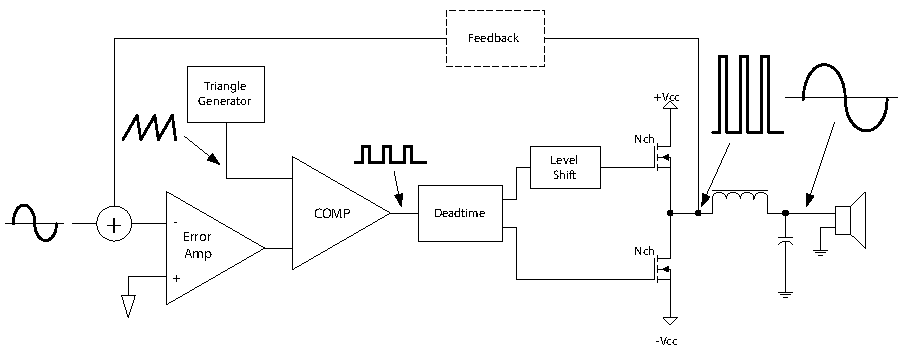
\includegraphics[width=\textwidth]{images/2_Preliminaries/Class-D Amplifier.pdf}
	\vspace{-0.2cm}
    \caption{Typical Class-D Amplifier \cite{analog_class_d_Basics}}
    \label{fig:class_d_amplifier}
\end{figure}
\newpage

\section{Quadrature Amplitude Modulation}\label{2_QAM_sec:QAM}
\acrfull{qam} \cite{nat_skript} is a modulation scheme where an in-phase component $I(t)$ and a quadrature component $Q(t)$ are mixed with orthogonal carriers and then added together, as shown in Figure \ref{2_fig:qam_diagram}. 
\begin{figure}[h!]
    \centering
    \includegraphics[width=0.5\textwidth]{images/2_Preliminaries/QAM.pdf}
    \caption{Block diagram \acrshort{qam}}
    \label{2_fig:qam_diagram}
\end{figure}

The output signal $f(t)$ can be calculated as 
\begin{equation}
    f(t) = I(t) \sin \left ( \omega_0 t\right ) + Q(t)\underbrace{\sin \left ( \omega_0 t + \frac{\pi}{2} \right)}_{\cos{(\omega_0 t)}}.
\end{equation}
Through the use of some trigonometric identities this can be simplified to 
\begin{equation}
    f(t) = \sqrt{I^2(t) + Q^2(t)} \sin{\left(\omega_0 t + \arctan{ \left ( \frac{Q(t)}{I(t)} \right )}. \right )}
\end{equation}
\section{Piezoelectric Ultrasonic Transducer}
\acrfull{put} emit sound by using the reciprocal piezoelectric effect \cite{air_coupled_ultraonic}. By applying an electric voltage to piezoelectric material it is deformed and therefore produces ultrasound. Electrically a \acrshort{put} is best described by using the Butterworth Van Dyke model, which is shown in Figure \ref{2_fig:butt_dyke_model}.
Of which the impedance response looks like Figure \ref{2_fig:impedance_put}.
\begin{figure}[h!]
    \centering
    \includegraphics[width=0.5\textwidth]{sections/Van_Dyke_Circuit.pdf}
    \caption{Butterworth van Dyke model}
    \label{2_fig:butt_dyke_model}
\end{figure}
\begin{figure}
    \centering
    \includegraphics[width=0.85\textwidth]{images/2_Preliminaries/Impedance_PUT.pdf}
    \caption{Magnitude of the impedance response \cite{air_coupled_ultraonic}}
    \label{2_fig:impedance_put}
\end{figure}


\section{Diffraction from slits}
The principle of Huygens-Fresnel \cite{physik_skript} states that every element on a wave surface can be viewed as a center of a spherical wave. Even if this is physically viewed not entirely correct, this provides a good model through which the wave changes in time can be calculated. This principle will be used to calculate the diffraction of waves on slits.

The calculations for the diffraction are only made in the far-field. 
\subsection{Single-Slit Diffraction}\label{2_subsec:single_slit}
All the points inside of the slits are viewed, accordingly to the huygens-fresnel principle, as centers of spherical waves. 
If we now want to know the pressure of a wave of frequency $\omega$ at a certain point in space, with distance r and angle $\phi$ to the slit, one can superposition all the points inside of the slit \cite{physik_skript}
\begin{equation}
    p(r, \phi, \omega)  
    = 
    \frac{A}{rs}\int_0^s \cos \left ( \omega t - k r + k x \sin\left ( \phi\right )\right) dx.
\end{equation}
Where A is the amplitude of the wave at the slit, s is the size of the slit and k is the wave number given as
\begin{equation}
    k 
    = 
    \frac{\omega}{c}
\end{equation}
This can be simplified to be
\begin{equation}
     p(r, \phi, \omega) 
     = 
     \frac{A}{r}  \underbrace{\frac{\sin \left ( \frac{ks \sin \phi}{2}\right )}{ \frac{ks \sin \phi}{2}}}_{A_s(\phi,k,s)} \cos \left ( \omega t - k r_s\right ).
     \label{2_eq:single_slid_final}
\end{equation}
The function $A_s(\phi,\omega,s)$ shows how the amplitude varies according to the angle, the frequency and the size of the slid. 

In Figure \ref{2_subfig:single_slid_amp} it is shown how the amplitude over the angle changes with different frequency while the slit size is hold constant at $s = 0.016 \,$m for waves with the speed $343 \,$m/s (speed of sound at 22 degrees Celsius). Additionally Figure \ref{2_subfig:single_slid_pow} shows the power. 
\begin{figure}
    \begin{minipage}{0.49\textwidth}
    \centering
    \includegraphics[width=\textwidth]{images/2_Preliminaries/Single_Slid_Frequency.pdf}
    \caption{Amplitude of waves with different frequencies}
    \label{2_subfig:single_slid_amp}
    \end{minipage}
    \begin{minipage}{0.49\textwidth}
    \centering
    \includegraphics[width=\textwidth]{images/2_Preliminaries/Single_Slid_Frequency_Power.pdf}
    \caption{Amplitude of waves with different frequencies}
     \label{2_subfig:single_slid_pow}
    \end{minipage}
\end{figure}

\subsection{Diffraction on Slits \& Fourier-Transform}\label{2_Acoustics_sec:diffraction_fourier}
Another way to calculate the diffraction pattern of a sound wave on slits is to take a kind of Fourier transform of this slits if the frequency is assume to be $\frac{k x}{2 \pi z}$.

For example in the case with one slit, which has a size of $s$ and and its middle is at the point $(0,0)$ and edges at $(0,\pm s/2)$ the "slit function" $a_s$ would look like
\begin{equation}
     a_s(x) =
    \begin{cases}
      1 & \text{$|x| < \frac{s}{2}$}\\
      0 & \text{else}
     \end{cases}
\end{equation}
Of which the Fourier transform would be
\begin{equation}
    \mathcal{F}\left \{ a_s(x) \right \} = A_s\left ( 2\pi\frac{f x}{c z} \right ) = s\frac{\sin{\left(  \frac{\pi f x s}{c z} \right )}}{\frac{\pi f x s}{c z}} 
\end{equation}
Near the x axis this can be simplified to
\begin{equation}
    \frac{x}{z} = \sin{(\varphi)}
\end{equation}
can be made. This leads to the same formula for the amplitude as seen before in \ref{2_eq:single_slid_final}
\begin{equation}
    A_s(\phi, k, s) = \frac{\sin \left ( \frac{ks \sin \phi}{2}\right )}{ \frac{ks \sin \phi}{2}}.
\end{equation}
\subsection{Multiple Slits Diffraction}
With the fourier transform idea, explained in \ref{2_Acoustics_sec:diffraction_fourier}, the amplitude and power of any multi-slit layout can now easily be calculated. For Z equally sized, $s$, and equally spaced, $d$, grid the pattern can be easily calculated to be
\begin{equation}
     A_s(\phi, k, s, d, Z)
     =
     \frac{\sin \left ( \frac{ks \sin \phi}{2}\right )}{ \frac{ks \sin \phi}{2}} \frac{\sin^2\left( \frac{k d \sin{\varphi}}{2}Z\right )}{\sin^2\left( \frac{k d \sin{\varphi}}{2}\right )}
\end{equation}
Where Z is the number of slits and d is their distance. In Figure \ref{6_fig:multiple_diffraction} an example of a diffraction at multiple slits with different spacing between them is shown.
\begin{figure}
    \centering
    \includegraphics[width=0.7\textwidth]{images/2_Preliminaries/Multiple_Slid_Count.pdf}
    \caption{Diffraction on multiple slits}
    \label{6_fig:multiple_diffraction}
\end{figure}

\newpage
\section{Acoustics}
\subsection{Basics}
A sound wave is a disturbance propagated through  a material (mostly air in acoustics) which causes a variation in pressure.
This disturbance in the ambient pressure is the sound pressure and is proportional to the inverse of the squared distance to the source.\cite{BERANEK20121}
\begin{equation}\label{2_Acoustics_eq:Pressure_sphere}
    p(r) \propto \frac{1}{r^2}.
\end{equation}
To get a better feeling for sound pressure in Table \ref{2_Acoustics_tab:Sound_pressure_level} are some examples of different sound sources, distances and their sound pressure. \cite{rossing1990science}
\begin{center}
\begin{table}[h!]
    \centering
    \begin{tabular}{| c | c | c | c |} 
     \hline 
     Sound source & Distance & Sound Pressure [Pa] & SPL [dB ref. 20$\mu$Pa] \\ 
     \hline
     Jet takeoff & 60$\,$m & 20 & 120 \\  
     Loud shouting & 1.5$\,$m & 2 & 100 \\
     Busy street & - & 0.2 & 80 \\
     Normal conversation & 1$\,$m & 0.02 & 60 \\
     Hearing threshold & - & 0.00002 & 0 \\
      \hline
    \end{tabular}
    \caption{Sound sources and their respective sound pressure (level)}
    \label{2_Acoustics_tab:Sound_pressure_level}
\end{table}
\end{center}
Additionally the sound pressure level (SPL) $L_p$ is displayed. It is the logarithmic measure of sound pressure $p$ relative to a reference value $p_0$.
\begin{equation}
    L_p 
    =
    20 \log_{10} \left ( \frac{p}{p_0} \right ) [dB].
\end{equation}
Mostly this reference value is picked to be $20 \, \mu\text{Pa}$ which is the hearing threshold for humans. \cite{rossing1990science}
\subsection{Sound Power}
The sound power is the total sound energy emitted by a loudspeaker. Often instead of the sound power the sound power level is used. This sound power level $L_W$ is the logarithmic measure of sound power $P$ relative to a reference power $P_0$
\begin{equation}
    L_W = 10\log_{10} \left (  \frac{P}{P_0} \right ) [dB].
\end{equation}
The reference power is often chosen to be $1 \, \text{pW}$. \cite{rossing1990science}
\subsection{Directivity}
In this application specially the directivity of a sound source is of high importance, due to the goal of creating a highly directional beam. 
The directivity of s a sound source is expressed as its directivity factor $Q_D$. It is definded as \cite{DirectivityIndices}
\begin{equation}\label{2_Acoustics_eq:Directivity}
    Q_D = \frac{|p_{axis}|^2}{\rho_0 c}\frac{4 \pi r^2}{W} = \frac{4 \pi p_{rms}^2}{2\pi\int_0^{\pi}p^2_{rms}(\theta)\sin{\theta}d\theta} 
\end{equation}
\subsection{Sound Power Level vs. Sound Pressure Level}
The sound pressure level at any point can be calculated through the distance to the source $r$, the sound power level of the source and the directivity and can be calculated, according to \cite{Relationship_Sound_pressure}, as
\begin{equation}\label{2_Acoustics_eq:SPLvSPL}
    L_p = L_W + 10\log_{10}\left( \frac{Q_D}{4 \pi r^2} + \frac{4}{R_c} \right ).
\end{equation}
Where $R_c$ is the room constant given as
\begin{equation}
    R_c = \frac{S\alpha_{av}}{1 - \alpha_{av}} [m^3].
\end{equation}
Here $S$ stands for the volume  and $\alpha_{av}$ is the average absorption coefficient of the room.  If the room is large enough ($S >> 1$) then $R_c >> 1$ follows which means Equation \ref{2_Acoustics_eq:SPLvSPL} can be simplified to
\begin{equation}
     L_p 
     = 
     L_W + 10\log_{10}\left( \frac{Q_D}{4 \pi r^2} \right ) 
     =
     L_W + 10\left ( \log_{10}(Q_D) - \log_{10}(r^2) - \underbrace{\log_{10}(4\pi)}_{\approx 1.1}  \right ). 
\end{equation}